\documentclass[a4paper]{article}            % Mind the a4paper option!
\usepackage[physuk,themered,noinnovation]{tuepdfscreen2008}        % winuk is the package option that displays the "Mathematics and Computer Science" logo
                                            % Other department options are:
                                            % ele, eleuk, bmt, bmtuk, bwk, bwkuk, id, iduk, chem, chemuk, tm, tmuk, phys, physuk, win, winuk, wtb, wtbuk
                                            % Options for handouts: handouts2, handouts3, handouts4, handouts6 and handouts8.
\usepackage[english]{babel}

\title{Machine Learning in Space Weather}                  % Title for title page
\author{Mandar Chandorkar}  % Subtitle for title page
\date{14 November 2019}  % status bar text for title page
%\titlelogo{mylogo}                                     % Uncomment this line to insert your own logo
\titlebackgroundimage[]{aurora.jpg}          % Background image for title page. The [bb=0 0 1554 1828] option specifies the size of
                                                              % the image, which is 1554 x 1828 pixels at 72 dpi. This option is usually not required,
                                                              % but it is only necessary if you have a JPG or PNG image AND want to LaTeX
                                                              % (instead of PDFLaTeX) your document.
\setstatustext{Mandar Chandorkar, November 2019}    % Status bar text for all pages except the title page.

\begin{document}

\begin{titleslide}
% You can put a sub-subtitle here if you like
\end{titleslide}

% \begin{slidetop}
% \tableofcontents
% \end{slidetop}


\begin{slidetop}
    \slidetitle{Eye of the Storm}
    \slidepictureleft[width=\textwidth]{Carrington_Richard_sunspots_1859.jpg}% The [bb=0 0 872 434] option specifies the size of
                                                                  % the image, which is 872 x 434 pixels at 72 dpi. This option is usually not required,
                                                                  % but it is only necessary if you have a JPG or PNG image AND want to LaTeX
                                                                  % (instead of PDFLaTeX) your document.
    
\end{slidetop}

\begin{slidetop}
    \slidetitle{Eye of the Storm}
    \slidepictureleft[width=\textwidth]{cme.jpg}% The [bb=0 0 872 434] option specifies the size of
                                                                  % the image, which is 872 x 434 pixels at 72 dpi. This option is usually not required,
                                                                  % but it is only necessary if you have a JPG or PNG image AND want to LaTeX
                                                                  % (instead of PDFLaTeX) your document.
    
\end{slidetop}

\begin{slidetop}
    \slidetitle{Space Weather}
    \slidepictureleft[width=\textwidth]{esa-sw.jpg}% The [bb=0 0 872 434] option specifies the size of
                                                                  % the image, which is 872 x 434 pixels at 72 dpi. This option is usually not required,
                                                                  % but it is only necessary if you have a JPG or PNG image AND want to LaTeX
                                                                  % (instead of PDFLaTeX) your document.
    
\end{slidetop}

\begin{slidetop}
    \slidetitle{Data Sources - Sun}
    \begin{center}
        \includegraphics[width=0.85\textwidth]{sdo.jpg}% The [bb=0 0 872 434] option specifies the size of
                                                                  % the image, which is 872 x 434 pixels at 72 dpi. This option is usually not required,
                                                                  % but it is only necessary if you have a JPG or PNG image AND want to LaTeX
                                                                  % (instead of PDFLaTeX) your document.
    \end{center}
    
\end{slidetop}

\begin{slidetop}
    \slidetitle{Data Sources - Earth}
    \slidepictureleft[width=\textwidth]{satellites-nasa.jpg}% The [bb=0 0 872 434] option specifies the size of
                                                                  % the image, which is 872 x 434 pixels at 72 dpi. This option is usually not required,
                                                                  % but it is only necessary if you have a JPG or PNG image AND want to LaTeX
                                                                  % (instead of PDFLaTeX) your document.
    
\end{slidetop}


\begin{slidetop}
    \slidetitle{Forecast with Uncertainty}
    \begin{center}
        \includegraphics[width=0.65\textwidth]{PredErrBars_Storm46.png}% The [bb=0 0 872 434] option specifies the size of
                                                                  % the image, which is 872 x 434 pixels at 72 dpi. This option is usually not required,
                                                                  % but it is only necessary if you have a JPG or PNG image AND want to LaTeX
                                                                  % (instead of PDFLaTeX) your document.    
    \end{center}
    
    
\end{slidetop}

\begin{slidetop}
    \slidetitle{Physics + ML}
    \begin{center}
        \includegraphics[width=0.65\textwidth]{prior_posterior_scatter_Q_alpha_b.png}% The [bb=0 0 872 434] option specifies the size of
                                                                  % the image, which is 872 x 434 pixels at 72 dpi. This option is usually not required,
                                                                  % but it is only necessary if you have a JPG or PNG image AND want to LaTeX
                                                                  % (instead of PDFLaTeX) your document.
    \end{center}
    
\end{slidetop}

\begin{slidetop}
    \slidetitle{Long Horizon Forecasts}
    \begin{center}
        \includegraphics[width=0.65\textwidth]{test_2016-11-16_2016-12-17_ts.pdf}% The [bb=0 0 872 434] option specifies the size of
                                                                  % the image, which is 872 x 434 pixels at 72 dpi. This option is usually not required,
                                                                  % but it is only necessary if you have a JPG or PNG image AND want to LaTeX
                                                                  % (instead of PDFLaTeX) your document.
    \end{center}
    
\end{slidetop}



\begin{slidetop}
    \slidetitle{Thank You!}
    \begin{center}
        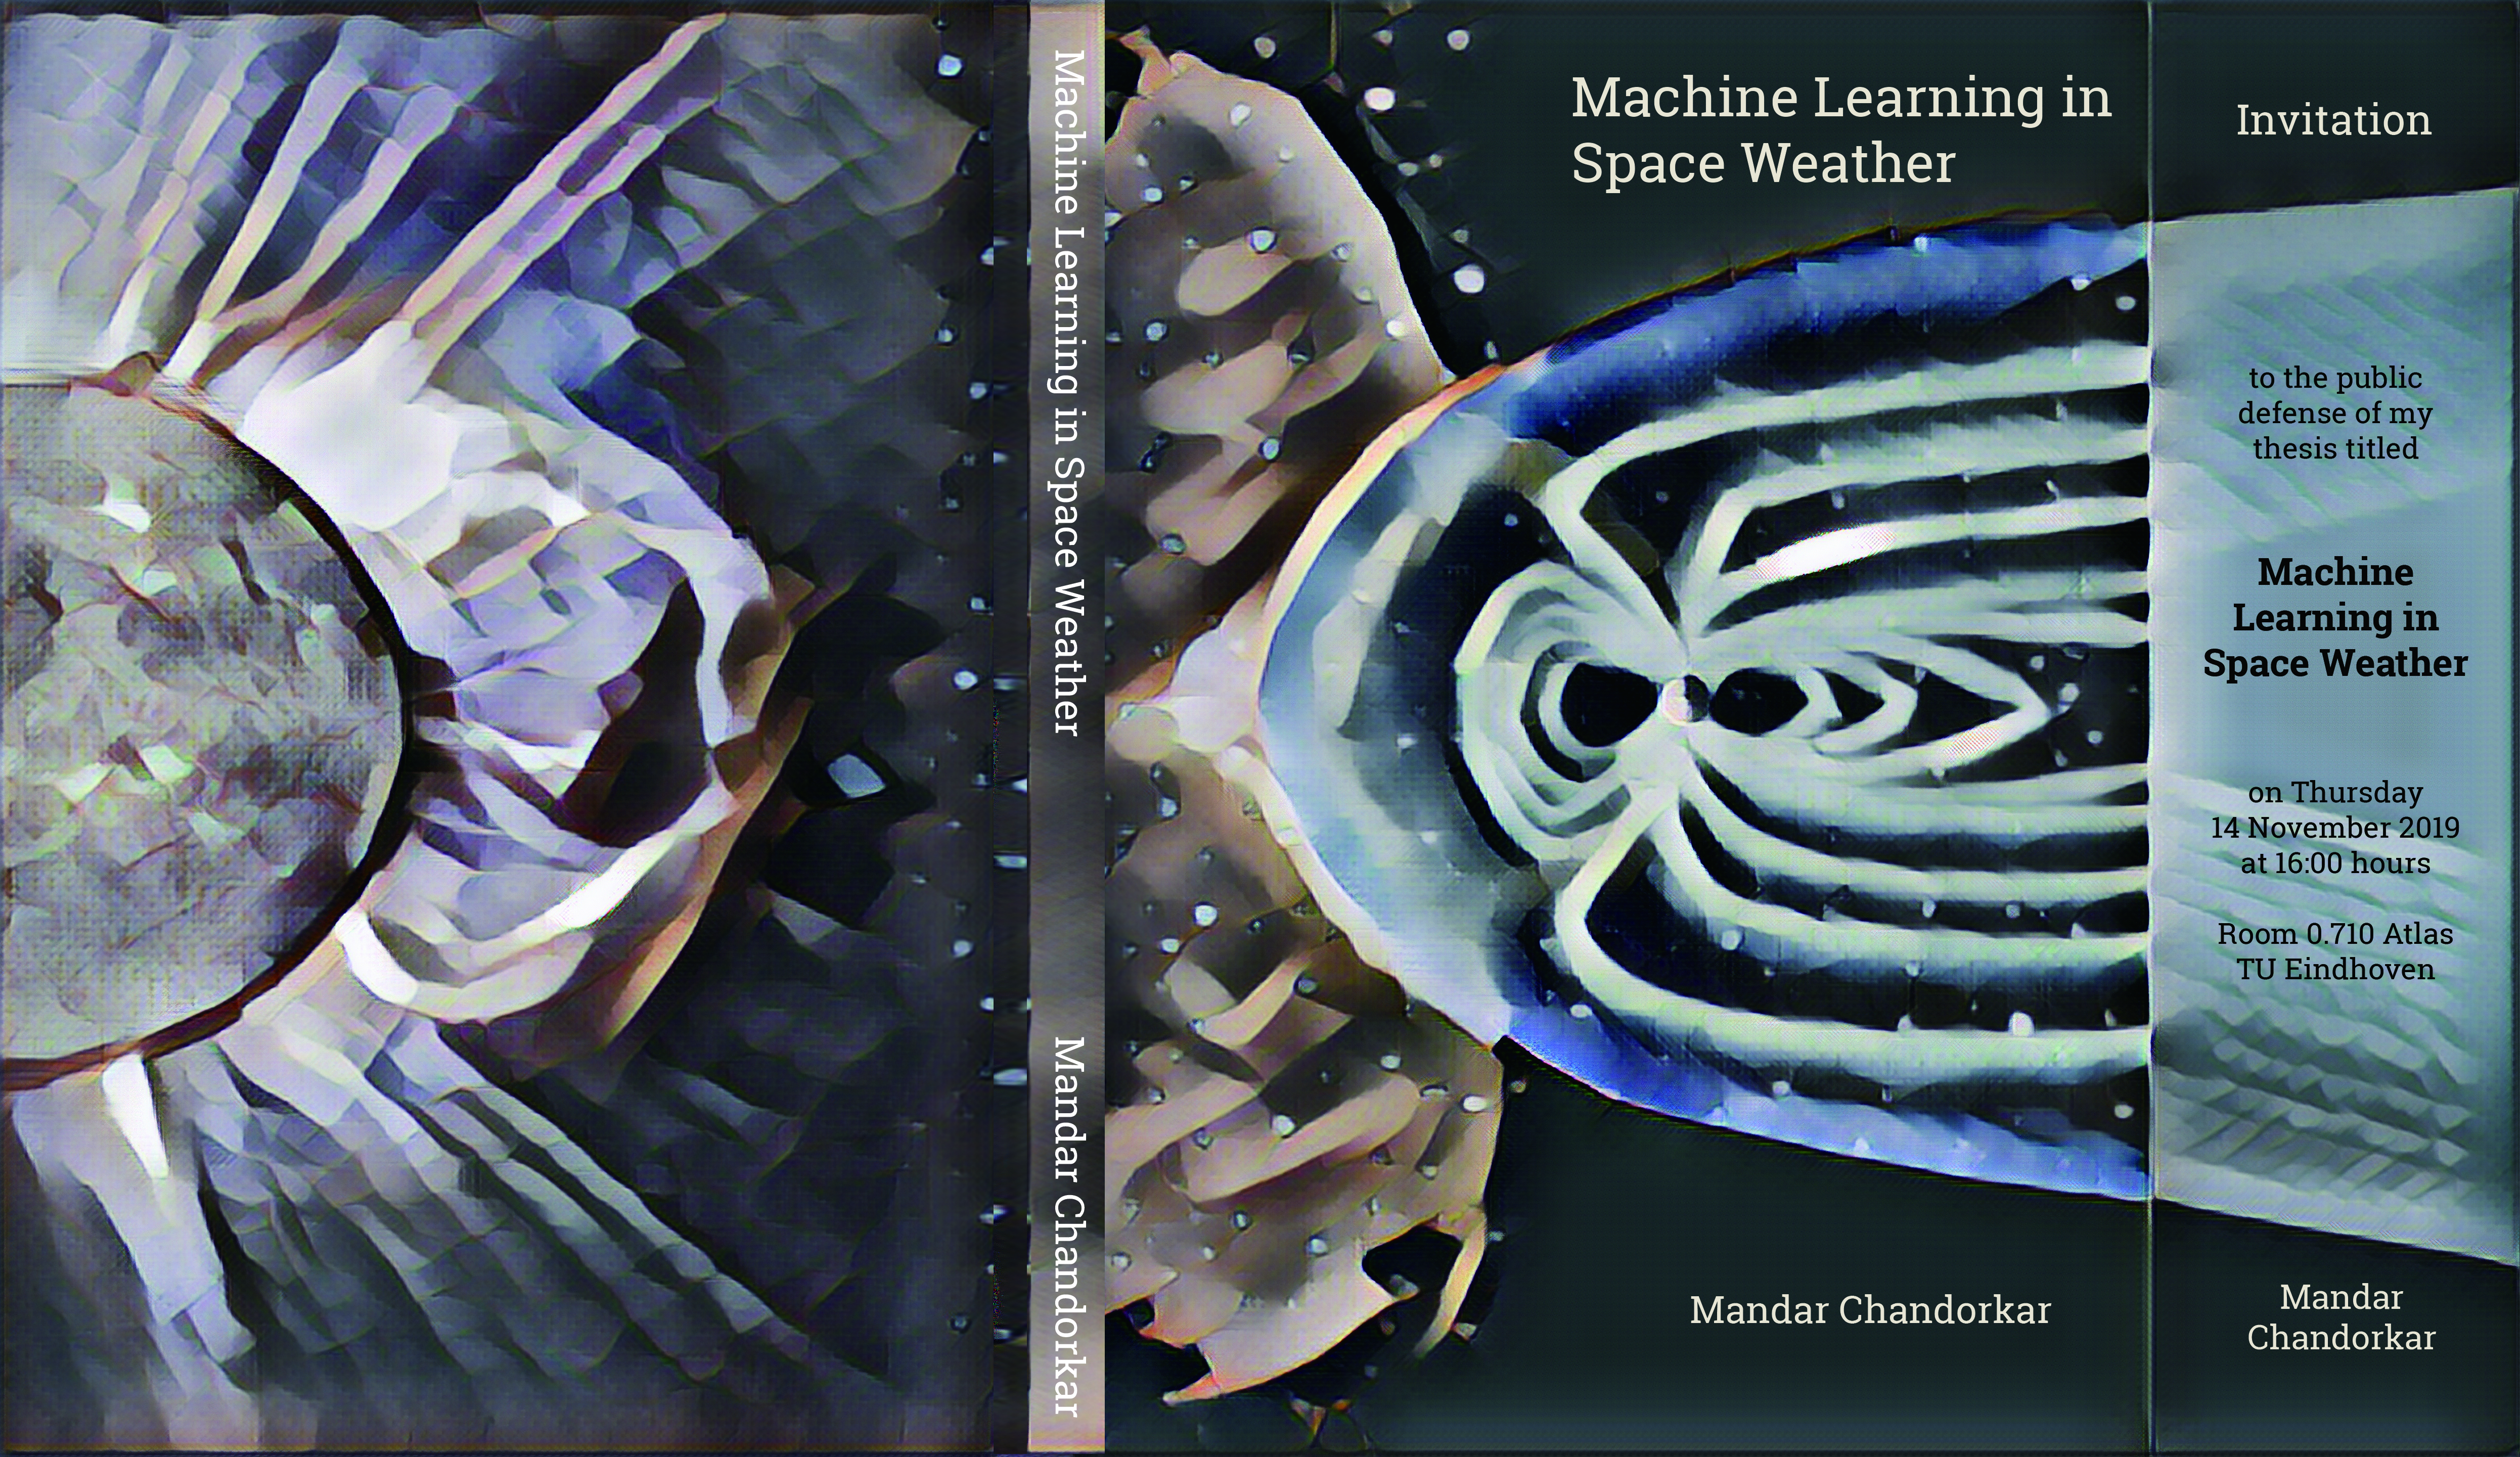
\includegraphics[width=\textwidth]{cover_3.jpg}% The [bb=0 0 872 434] option specifies the size of
                                                                  % the image, which is 872 x 434 pixels at 72 dpi. This option is usually not required,
                                                                  % but it is only necessary if you have a JPG or PNG image AND want to LaTeX
                                                                  % (instead of PDFLaTeX) your document.
    \end{center}
    
\end{slidetop}


% \begin{slidetop}
% \slidetitle{TU/e corporate identity}      % The \slidetitle command creates a slide title without adding it to the table of contents
% \slidepictureright[bb=0 0 324 434]{tueimg1.jpg}               % The [bb=0 0 324 434] option specifies the size of
%                                                               % the image, which is 324 x 434 pixels at 72 dpi. This option is usually not required,
%                                                               % but it is only necessary if you have a JPG or PNG image AND want to LaTeX
%                                                               % (instead of PDFLaTeX) your document.


% \begin{minipage}{12cm}   % 12cm is the width of the minipage in which the text is placed. You have to adjust this length manually depending on the width of your picture
% \section*{Page with text and picture}

% This slide shows how to put both text and an image next to each other in one slide. Unfortunately you have to use a \verb|minipage| to specify the width of the text next to the image.

% The next slide shows a slide which is filled completely with one picture. To obtain the best results, make sure that the aspect ratio of your picture is approximately 2 : 1 (width : height).
% \end{minipage}
% \end{slidetop}


\end{document}
